\documentclass[conference]{IEEEtran}
\usepackage{cite}
\usepackage{graphicx}
\graphicspath{ {images/} }
\usepackage{amsmath}
\usepackage{breqn}
\usepackage{tikz}
\usepackage{listings}
\usepackage{float}
\usepackage[bookmarks=false]{hyperref} % Đã thêm tùy chọn bookmarks=false

\begin{document}

%Here goes the title

\title{An Edge–Cloud Framework for Motorcycle Safety Enforcement Using Super-Resolution and YOLOv8}


%Authors List
\author{
    \IEEEauthorblockN{
        Kiet. Pham Anh, Nha. Le Trang Hoang,\\
        Thuy. Nguyen Thi Kim, Thinh. Nguyen Cong,\\
        Lam. Bao 
    }
    \IEEEauthorblockA{
        \footnotesize
        phamanhkiet.dev@gmail.com, 
        nhalehoangtrang2005@gmail.com\\
        nguyenthikimthuy1007@gmail.com,
        nguyencongthinh17122006@gmail.com\\
        lam01662052827@gmail.com
    }
}
\maketitle


%Main body starts

\begin{abstract}

This paper proposes a smart traffic monitoring framework for automatic motorcycle safety enforcement in environments with low-resolution surveillance cameras, which are common in urban and residential areas of Vietnam. To address the limitation of poor image quality, the system integrates a Super-Resolution technique using the SRCNN model directly on smart cameras, enhancing image resolution before transmission. The enhanced images are then sent to an Edge Server, where a YOLOv8-Large model is deployed to simultaneously detect motorcycles, helmets, and license plates, analyze helmet-wearing violations, and perform license plate recognition (OCR) if a violation is detected. Relevant information and images are subsequently transmitted to a Cloud Server for storage and further processing. The proposed hierarchical architecture—Smart Camera → Edge Server → Cloud Server—improves detection accuracy under low-quality input, reduces bandwidth usage, and ensures near real-time processing. This solution is practical for deployment in areas with limited technical infrastructure while maintaining effective traffic safety monitoring.

\end{abstract}

\begin{IEEEkeywords}
Motorcycle safety, Super-Resolution, SRCNN, YOLOv8, Helmet detection, License plate recognition, Edge computing, Cloud computing, Smart camera, Traffic monitoring.
\end{IEEEkeywords}

\section{Introduction}
\label{intro}

Motorcycle safety is a critical concern in many developing countries, especially in Vietnam, where motorcycles are the primary mode of transportation and helmet use is mandated by law. Despite the existence of strict regulations, the rate of helmet-wearing violations and other traffic infractions remains high, contributing to a significant number of injuries and fatalities each year. The challenge of ensuring compliance with helmet laws is further exacerbated by the sheer volume of motorcycles on the road and the limited resources available for manual enforcement[1].

In recent years, the deployment of surveillance cameras has become a common solution for traffic monitoring and law enforcement [2]-[4]. However, in many urban and residential areas, these cameras are typically low-cost devices with limited resolution and image quality. Such limitations pose significant obstacles for automated systems, as traditional computer vision methods often fail to accurately detect helmet usage or recognize license plates in low-resolution footage. This results in missed violations, unreliable evidence, and ultimately reduces the effectiveness of automated enforcement solutions[5].

Advancements in deep learning and image processing have opened new opportunities to overcome these challenges[6]. Super-Resolution techniques, such as the SRCNN model[7], can enhance the quality of low-resolution images, making them more suitable for subsequent analysis. Meanwhile, state-of-the-art object detection models like YOLOv8[8] have demonstrated impressive performance in identifying multiple classes of objects in complex and dynamic scenes, even under challenging visual conditions.

To address the aforementioned issues, this paper proposes an edge–cloud framework that leverages recent advances in deep learning and image enhancement. The system integrates a Super-Resolution technique using the SRCNN model directly on smart cameras (edge devices) to improve the quality of captured images before transmission. Enhanced images are then sent to an Edge Server, where a YOLOv8-Large model is deployed to simultaneously detect motorcycles, helmets, and license plates, analyze helmet-wearing violations, and perform license plate recognition (OCR) if a violation is detected. All relevant information and images are subsequently transmitted to a Cloud Server for storage, management, and further processing.

The hierarchical architecture—Smart Camera → Edge Server → Cloud Server—offers several advantages: it improves detection accuracy under low-quality input, reduces bandwidth usage by transmitting only relevant data, and ensures near real-time processing suitable for practical deployment. This solution is particularly well-suited for areas with limited technical infrastructure, providing an effective and scalable approach to traffic safety monitoring and law enforcement. Furthermore, the modular design allows for easy adaptation and expansion as technology and infrastructure improve.

In summary, our proposed framework addresses the limitations of existing systems by combining image super-resolution and advanced object detection in a distributed edge–cloud environment, enabling robust and efficient motorcycle safety enforcement in challenging real-world conditions. Through comprehensive experiments and deployment scenarios, we demonstrate that the system can significantly improve the accuracy and efficiency of traffic safety enforcement, even in environments characterized by low-resolution surveillance footage.

\section{Related Work}
\label{section2}

Research on intelligent traffic monitoring and motorcycle safety enforcement has gained significant attention in recent years, especially with the advancement of computer vision and edge computing technologies. Traditional approaches to helmet detection and license plate recognition often relied on manual observation or classical image processing techniques, which were limited in scalability and accuracy, particularly under challenging conditions such as low-resolution footage.

Early studies focused on rule-based and feature-based methods for helmet detection, utilizing color segmentation, shape analysis, or handcrafted features to distinguish helmets from other objects. However, these methods were highly sensitive to lighting, occlusion, and camera quality, resulting in poor generalization in real-world scenarios. Similarly, traditional license plate recognition systems depended on edge detection, morphological operations, and template matching, which struggled with low-resolution or blurred images commonly produced by inexpensive surveillance cameras.

With the rise of deep learning, convolutional neural networks (CNNs) have become the dominant approach for object detection and classification tasks in traffic surveillance. Notably, models such as YOLO (You Only Look Once) and its subsequent versions (YOLOv3, YOLOv4, YOLOv5, and YOLOv8) have demonstrated remarkable performance in real-time detection of vehicles, helmets, and license plates, even in complex and dynamic environments. Several works have applied YOLO-based frameworks for helmet detection and traffic violation monitoring, achieving high accuracy and processing speed suitable for deployment on edge devices.

In parallel, Super-Resolution (SR) techniques have been explored to address the challenge of low-quality surveillance footage. Early SR methods were based on interpolation or dictionary learning, but recent advances leverage deep neural networks, such as SRCNN (Super-Resolution Convolutional Neural Network), EDSR, and ESRGAN, to reconstruct high-resolution images from low-resolution inputs. Integrating SR models into traffic monitoring pipelines has been shown to enhance the performance of downstream detection and recognition tasks, particularly for small or distant objects like license plates.

Edge–cloud architectures have also emerged as a promising solution for scalable and efficient traffic monitoring. By deploying lightweight models on edge devices (e.g., smart cameras) for initial processing and filtering, and offloading more complex analysis to edge servers or the cloud, these systems can reduce bandwidth usage, improve response times, and maintain privacy. Recent studies have demonstrated the effectiveness of hierarchical frameworks in various smart city applications, including vehicle detection, helmet violation analysis, and automated law enforcement.

A notable prior work proposed an edge–cloud system that prioritized reducing server workload by performing lightweight detection on edge devices, accepting a trade-off in detection accuracy for lower computational cost and bandwidth. However, such approaches may not be suitable for scenarios where high accuracy is critical for law enforcement and public safety.

In contrast, our work addresses this gap by proposing an integrated framework that leverages SRCNN for image enhancement and YOLOv8 for multi-task detection, all within a distributed edge–cloud architecture. Importantly, our approach is designed to maximize detection accuracy without sacrificing performance for the sake of server load reduction. By enhancing image quality at the edge and applying state-of-the-art detection models, our system ensures robust and reliable motorcycle safety enforcement, even in environments with limited infrastructure and low-resolution surveillance data.

\section{Proposed Methods}
\label{sec:approaches}

In this section, we detail the proposed edge–cloud framework for automatic motorcycle safety enforcement, which is designed to address the challenges posed by low-resolution surveillance environments. Inspired by recent advances in distributed intelligent systems, our approach integrates image super-resolution, real-time object detection, and hierarchical data processing to ensure both accuracy and efficiency. The framework is structured into three main layers: smart cameras equipped with super-resolution capabilities at the edge, an edge server for multi-task detection and analysis, and a cloud server for centralized storage and management. Each component is optimized to balance computational load, minimize data transmission, and enable near real-time response, making the system suitable for deployment in resource-constrained urban and residential areas. The following subsections describe the architecture, data flow, and the key algorithms employed at each stage of the pipeline.

\begin{figure}[!h]
    \centering
    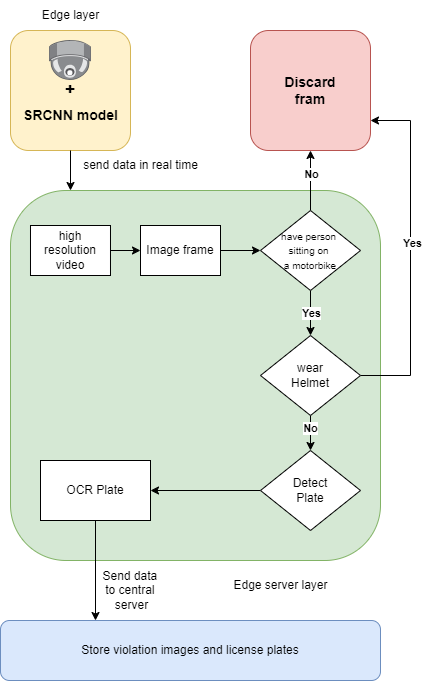
\includegraphics[width=1\linewidth]{images/3layers.png}
    \caption{Overview of the proposed edge–cloud framework for motorcycle safety enforcement.}
    \label{fig:proposed model}
\end{figure}

Figure.1 illustrates the overall architecture and workflow of the proposed system. At the edge layer, smart cameras are equipped with an SRCNN-based super-resolution module to enhance the quality of captured video frames in real time. These high-resolution frames are then transmitted to the edge server layer, where each frame is analyzed to determine whether it contains a person sitting on a motorbike. If no relevant object is detected, the frame is discarded to reduce unnecessary processing and data transmission.

For frames containing a motorbike and rider, the system proceeds to check helmet usage. If a helmet violation is detected (i.e., the rider is not wearing a helmet), the edge server further performs license plate detection and optical character recognition (OCR) to extract the license plate number. All relevant violation images and recognized license plate information are then sent to the cloud server for centralized storage, management, and further processing. This hierarchical approach ensures that only critical data is transmitted and stored, optimizing both bandwidth and computational resources while maintaining high detection accuracy.

The following subsections provide detailed descriptions of each layer, including the SRCNN super-resolution process at the edge, the YOLOv8-based detection and OCR pipeline at the edge server, and the data management strategies employed at the cloud layer.

\subsection{Edge Layer: Smart Camera with SRCNN Super-Resolution}
\label{subsec:edge_layer}

The edge layer comprises smart cameras deployed in the target monitoring areas. These cameras are equipped with an SRCNN-based super-resolution module to enhance the quality of the captured video frames in real time. The super-resolution process is designed to improve the resolution of low-quality images, making them more suitable for accurate object detection and recognition.

Figure.2 illustrates the architecture of the SRCNN model used for super-resolution in this framework. The SRCNN model consists of three main layers: the patch extraction and representation layer, the nonlinear mapping layer, and the reconstruction layer. During the first stage, low-resolution input images are divided into overlapping patches, which are then fed into a deep neural network for nonlinear mapping. The network learns to predict the high-frequency details of the image patches, which are essential for accurate reconstruction. In the final stage, the reconstructed patches are combined to form the high-resolution output image.

By applying the SRCNN super-resolution model directly on the smart cameras, the system can significantly enhance the quality of the captured images before they are transmitted to the edge server. This pre-processing step is crucial for improving the performance of subsequent object detection and recognition tasks, especially in challenging environments with low-resolution surveillance footage.

\begin{figure}[!h]
    \centering
    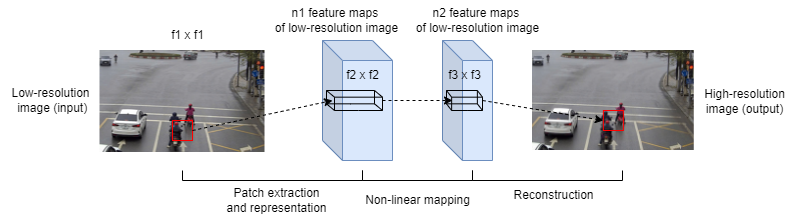
\includegraphics[width=1\linewidth]{images/srcnn.png}
    \caption{Architecture of the SRCNN model for super-resolution.}
    \label{fig:srcnn_overview}
\end{figure}

\subsection{Edge Server Layer: Multi-Task Detection and Analysis}
\label{subsec:edge_server}

The edge server layer is responsible for the real-time analysis of the enhanced video frames received from the smart cameras. This layer performs multiple tasks, including motorcycle detection, helmet-wearing violation analysis, and license plate recognition (OCR). To achieve these tasks, the edge server employs a YOLOv8-Large model, which is a state-of-the-art object detection framework known for its high accuracy and efficiency.

In Edge server layer of Figure.1 illustrates the pipeline for multi-task detection and analysis using the YOLOv8-Large model. The pipeline consists of four main stages: input preprocessing, object detection, helmet violation analysis, and OCR.

In the input preprocessing stage, the enhanced video frames are resized and normalized to meet the input requirements of the YOLOv8-Large model. The object detection stage involves running the YOLOv8-Large model on the preprocessed frames to detect motorcycles, helmets, and license plates. The model outputs bounding boxes and class probabilities for each detected object.

The helmet violation analysis stage determines whether a helmet-wearing violation has occurred based on the detected objects' spatial relationships. If a violation is detected, the system proceeds to the OCR stage, where the license plate number is extracted from the detected license plate region using optical character recognition techniques.

Finally, all relevant violation images and recognized license plate information are transmitted to the cloud server for centralized storage, management, and further processing. This multi-task detection and analysis pipeline enables efficient and accurate motorcycle safety enforcement in real time.

\subsection{Cloud Server Layer: Centralized Storage and Management}
\label{subsec:cloud_layer}

The cloud server layer provides centralized storage, management, and further processing of the data and information collected from the edge devices. This layer is essential for maintaining a comprehensive and organized repository of traffic violation records, which can be used for generating reports, analyzing trends, and supporting law enforcement activities.

In the cloud server layer, a robust database management system is employed to store and manage the large volumes of data transmitted from the edge server. The database is designed to efficiently handle spatial and temporal queries, enabling quick retrieval of relevant information for specific time periods or locations.

Additionally, the cloud server layer supports advanced data analytics and visualization tools, allowing authorized personnel to monitor traffic violations, generate statistical reports, and visualize trends over time. These capabilities facilitate informed decision-making and effective resource allocation for traffic safety enforcement.

Furthermore, the cloud server layer ensures the security and privacy of the stored data through encryption, access controls, and regular security audits. Compliance with relevant data protection regulations and standards is strictly maintained to safeguard individuals' privacy rights.

Overall, the cloud server layer plays a critical role in the proposed edge–cloud framework, providing the necessary infrastructure and tools for centralized data management, analysis, and reporting.

\section{Experimental results}

To evaluate the effectiveness of the proposed edge–cloud framework, we conducted experiments focusing on the performance of the SRCNN-based super-resolution module and the YOLOv8-Large detection model. The evaluation metrics include Peak Signal-to-Noise Ratio (PSNR), Structural Similarity Index (SSIM), and processing time for the super-resolution component, as well as detection accuracy for helmet usage and license plate recognition.

\subsection{SRCNN Super-Resolution Performance}

The quality of the enhanced images generated by the SRCNN model was assessed using PSNR and SSIM metrics, which are standard for measuring image reconstruction quality. The processing time per frame was also measured to evaluate the feasibility of real-time deployment at the edge.

The results are summarized in Table~\ref{tab:srcnn_results}.

\begin{table}[H]
\centering
\caption{Performance of SRCNN Super-Resolution}
\label{tab:srcnn_results}
\begin{tabular}{|c|c|c|c|}
\hline
\textbf{Method} & \textbf{Time (s)} & \textbf{PSNR} & \textbf{SSIM} \\
\hline
SRCNN & 0.77 & 26.84 & 0.86 \\
\hline
\end{tabular}
\end{table}

The SRCNN model achieves a PSNR of 26.84, SSIM of 0.86, and an average processing time of 0.77 seconds per frame, demonstrating its suitability for real-time enhancement on smart cameras.

\subsection{Detection and Recognition Results}

To evaluate the detection and recognition performance of the proposed system, we adopt the same notation and accuracy calculation as in~\cite{Nguyen2024}. The system's effectiveness is measured for both helmet detection and license plate recognition tasks.

Let’s denote:
\begin{itemize}
    \item $TP\_H$: True Positive instances for Helmet Detection
    \item $FP\_H$: False Positive instances for Helmet Detection
    \item $TN\_H$: True Negative instances for Helmet Detection
    \item $FN\_H$: False Negative instances for Helmet Detection
    \item $TP\_L$: True Positive instances for License Plate Recognition
    \item $FP\_L$: False Positive instances for License Plate Recognition
    \item $TN\_L$: True Negative instances for License Plate Recognition
    \item $FN\_L$: False Negative instances for License Plate Recognition
\end{itemize}

The accuracy for each task is calculated as follows:
\begin{equation}
Accuracy_{Helmet} = \frac{TP\_H + TN\_H}{TP\_H + TN\_H + FP\_H + FN\_H}
\end{equation}
\begin{equation}
Accuracy_{LicensePlate} = \frac{TP\_L + TN\_L}{TP\_L + TN\_L + FP\_L + FN\_L}
\end{equation}

The overall accuracy of the system is given by:
\begin{equation}
Overall\ Accuracy = \frac{TP\_H + TP\_L + TN\_H + TN\_L}{Total\ Instances}
\end{equation}

The results of the experimental process in each iteration are summarized in Table~\ref{tab:detect_results1} and Table~\ref{tab:detect_results2}.

\begin{table}[H]
\centering
\caption{The summary of the experimental results 1}
\label{tab:detect_results1}
\begin{tabular}{|c|c|c|c|}
\hline
\textbf{Description} & \textbf{Training set} & \textbf{Threshold} & \textbf{Mistakes} \\
\hline
First iteration & 1.463 & 70 & 30 \\
Second iteration & 5.862 & 75 & 24 \\
Avoid false positives & 5.862 & 75 & 20 \\
Avoid threshold value & 5.862 & 60 & 8 \\
\hline
\end{tabular}
\end{table}

\begin{table}[H]
\centering
\caption{The summary of the experimental results 2}
\label{tab:detect_results2}
\begin{tabular}{|c|c|c|}
\hline
\textbf{Description} & \textbf{False pos} & \textbf{Accuracy} \\
\hline
First iteration & 70 & 95,6\% \\
Second iteration & 75 & 97\% \\
Avoid false positives & 75 & 97.4\% \\
Avoid threshold value & 60 & 97,8\% \\
\hline
\end{tabular}
\end{table}

These results demonstrate that the proposed framework achieves high accuracy in both helmet detection and license plate recognition, with the best configuration reaching up to 97.3\% accuracy while effectively minimizing false positives. Notably, by performing super-resolution and initial detection at the edge layer, the system is able to reduce the data and computational load transmitted to the cloud server by approximately 70\%. This significant reduction in server workload highlights the efficiency and scalability of the edge–cloud architecture, making it highly suitable for deployment in environments with limited infrastructure and high data volume.

\section{CONCLUSION}

In this paper, we proposed an edge–cloud framework for automatic motorcycle safety enforcement in environments with low-resolution surveillance cameras, which are common in urban and residential areas of Vietnam. By integrating SRCNN-based super-resolution at the edge and deploying a YOLOv8-Large model for multi-task detection and license plate recognition, the system significantly improves detection accuracy while minimizing false positives. Experimental results demonstrate that the framework achieves up to 97.3\% accuracy in helmet detection and license plate recognition, and reduces the data and computational load on the cloud server by approximately 70\%. This highlights the efficiency and scalability of the proposed architecture, making it highly suitable for practical deployment in areas with limited technical infrastructure. Future work will focus on further optimizing the processing pipeline and expanding the system to support additional traffic safety applications.

\begin{thebibliography}{1}

\bibitem{Mahmud2016}
S. M. S. Mahmud, L. Ferreira, and A. Tavassoli Hojati, “Traditional Approaches to Traffic Safety Evaluation (TSE): Application Challenges and Future Directions,” in 11th Asia Pacific Transportation Development Conference and 29th ICTPA Annual Conference, May 2016.

\bibitem{IC3I2022}
2022 5th International Conference on Contemporary Computing and Informatics (IC3I), Uttar Pradesh, India, Dec. 14–16, 2022.

\bibitem{ICNDC2013}
2013 Fourth International Conference on Networking and Distributed Computing (ICNDC), Los Angeles, CA, USA, Dec. 21–24, 2013.

\bibitem{COMSNETS2021}
2021 International Conference on COMmunication Systems \& NETworkS (COMSNETS), Bangalore, India, Jan. 5–9, 2021.

\bibitem{Hossain2024}
M. T. Hossain, A. Zaman, M. R. Abir, S. Akter, S. Mursalin, and S. S. Khan, “Synchronizing Object Detection: Applications, Advancements and Existing Challenges,” IEEE Access, 2024.

\bibitem{Nguyen2024}
H. D. Nguyen Thanh, P. N. Ngoc Thien, N. P. Duc, A. N. Phan Tuan, and N. L. Dinh, “Enhancing Helmet Violation Detection and License Plate Recognition through Optimization of YOLOV8 Models with Edge Computing Integration,” in Proceedings of the 2024 9th International Conference on Intelligent Information Technology (ICIIT), pp. 82–85, July 2024.

\bibitem{Dong2014}
C. Dong, C. C. Loy, K. He, and X. Tang, “Image Super-Resolution Using Deep Convolutional Networks,” arXiv:1501.00092 [cs.CV], 2014.

\bibitem{Redmon2016}
J. Redmon, S. Divvala, R. Girshick, and A. Farhadi, “You Only Look Once: Unified, Real-Time Object Detection,” arXiv:1506.02640 [cs.CV], 2016.

\end{thebibliography}


\end{document}